\section{Huffman schedules}\label{sec:huffman}

When the soundness of a run is the reciprocal of an integer and the budget is a power of it, the optimal schedule is not only close to the entropy bound but computable exactly, and it is a code.

\subsection{Schedules are codes}

A $D$-ary \emph{prefix code} for $n$ symbols is a set of $n$ words over an alphabet of $D$ letters, none a prefix of another. Kraft's inequality says that lengths $\ell_{1},\dots,\ell_{n}\in\NN$ are the lengths of a prefix code if and only if $\sum_{i}D^{-\ell_{i}}\le1$ \cite{Kra49}, and McMillan's theorem extends the necessity to all uniquely decodable codes \cite{McM56}; Appendix~\ref{app:kraft} recalls the proofs. For a probability vector $p$ write $L_{D}(p)$ for the least value of $\sum_{i}p_{i}\ell_{i}$ over lengths satisfying Kraft's inequality, and $H_{D}(p)=H(p)/\log D$.

\begin{lemma}[Kraft form of soundness]\label{lem:kraftsound}
Let $D>1$ and $k\in\NN$, and let $r\in\NN^{n}$.
\begin{enumerate}[label=\textup{(\roman*)},leftmargin=2.2em,itemsep=1pt]
\item If $\sum_{i}D^{-r_{i}}\le D^{-k}$, then $r_{i}\ge k$ for every $i$ and $\ell_{i}=r_{i}-k$ satisfies $\sum_{i}D^{-\ell_{i}}\le1$.
\item If $\sum_{i}D^{-\ell_{i}}\le1$, then $r_{i}=\ell_{i}+k$ satisfies $\sum_{i}D^{-r_{i}}\le D^{-k}$.
\item $\sum_{i}a_{i}(\ell_{i}+k)=kA+\sum_{i}a_{i}\ell_{i}$.
\end{enumerate}
\end{lemma}

\begin{proof}
(i) Each term satisfies $D^{-r_{i}}\le\sum_{j}D^{-r_{j}}\le D^{-k}$, and $x\mapsto D^{-x}$ is decreasing, so $r_{i}\ge k$; then $\sum D^{-(r_{i}-k)}=D^{k}\sum D^{-r_{i}}\le1$. (ii) $\sum D^{-(\ell_{i}+k)}=D^{-k}\sum D^{-\ell_{i}}\le D^{-k}$. (iii) is linearity.
\end{proof}

\begin{proof}[Proof of Theorem~\ref{thm:C}]
With $\eps=1/D$ and $\theta=D^{-k}$, the $\theta$-sound schedules are the $r$ with $\sum D^{-r_{i}}\le D^{-k}$. By Lemma~\ref{lem:kraftsound} they are exactly the vectors $\ell+k$ with $\ell$ satisfying Kraft's inequality, which by Kraft's theorem are the length vectors of prefix codes. The cost is $kA+\sum a_{i}\ell_{i}=A(k+\sum p_{i}\ell_{i})$, and its minimum is $A(k+L_{D}(p))$. Huffman's algorithm produces a prefix code of expected length $L_{D}(p)$ (Appendix~\ref{app:huffman}).
\end{proof}

So the optimal schedule is obtained by building the Huffman tree of the cost profile and adding $k$ runs to every check (Fig.~\ref{fig:kraft}). Each run of a check is a letter of the codeword of its candidate; the first $k$ letters buy the budget $D^{-k}$, the remaining $\ell_{i}$ letters distinguish the candidate from the others, and a candidate of high cost gets a short word, as a frequent symbol does.

\begin{figure*}[t]
\centering
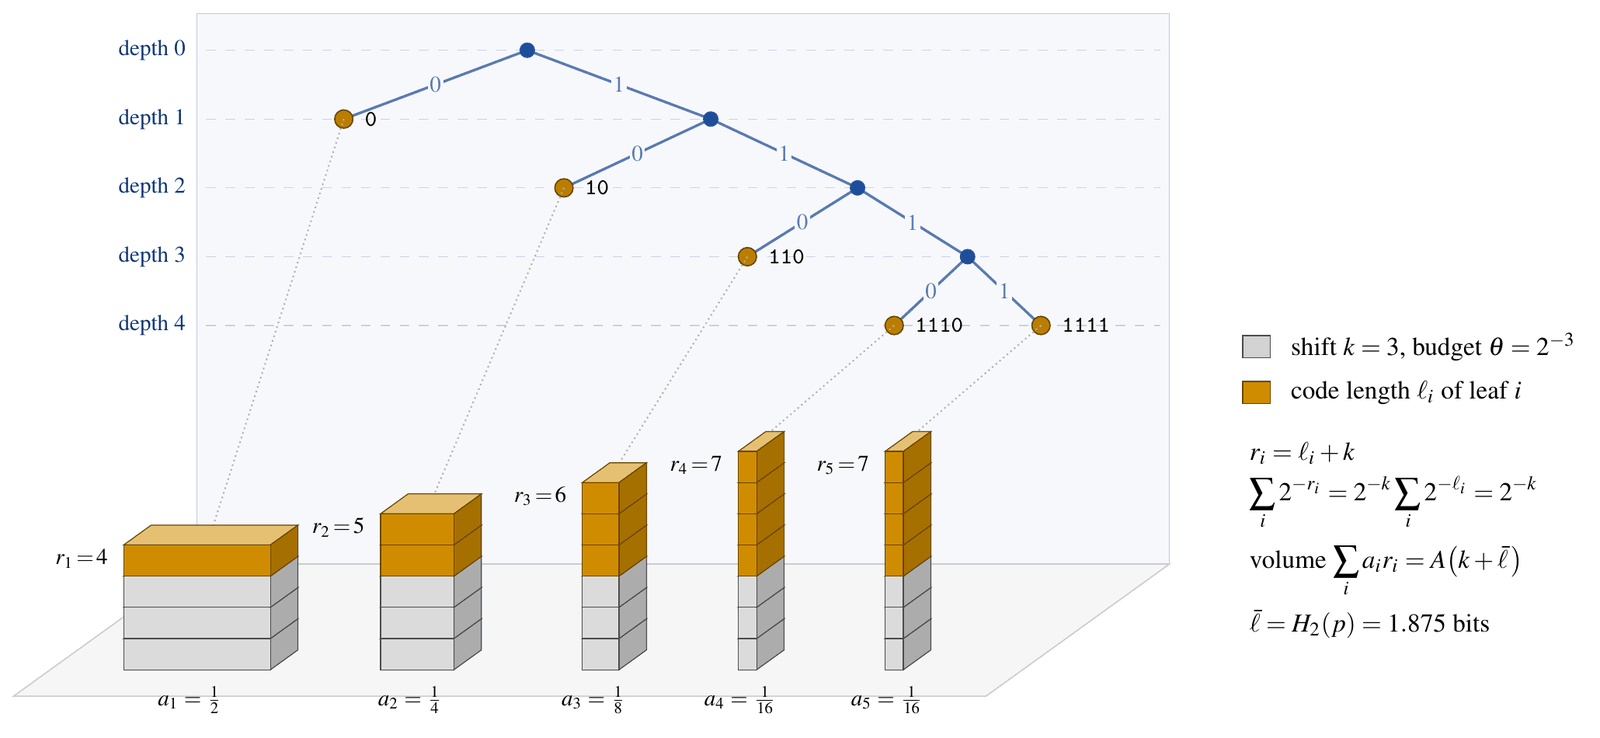
\includegraphics[width=0.92\textwidth]{figures/fig_kraft3d}
\caption{Theorem~\ref{thm:C} for the profile $p=(\frac12,\frac14,\frac18,\frac1{16},\frac1{16})$, $\eps=\frac12$ and $\theta=2^{-3}$. Back wall: the binary Huffman tree, with codewords $0$, $10$, $110$, $1110$, $1111$. Floor: a column for each candidate, of width proportional to its cost $a_{i}$, built from $k=3$ grey blocks, which buy the budget $2^{-3}$, and $\ell_{i}$ gold blocks, one per letter of its codeword. The heights are the optimal numbers of runs $r_{i}=4,5,6,7,7$, the budget is exactly spent, $\sum2^{-r_{i}}=2^{-3}$, and the volume of the columns is the optimal cost $A(k+\bar\ell)$ with $\bar\ell=H_{2}(p)=1.875$.}
\label{fig:kraft}
\end{figure*}

\begin{corollary}\label{cor:huffbounds}
Under the hypotheses of Theorem~\ref{thm:C}, $A(k+H_{D}(p))\le\Vs(D^{-k})<A(k+H_{D}(p)+1)$, with equality on the left if and only if every $p_{i}$ is an integer power of $1/D$.
\end{corollary}

\begin{proof}
Shannon's bounds $H_{D}(p)\le L_{D}(p)<H_{D}(p)+1$ \cite{Sha48,CT06} are the case $\theta=1$ of Theorem~\ref{thm:A}, since $L=\log D$ and $(A/L)H(p)=AH_{D}(p)$; the equality case is that of Proposition~\ref{prop:entropyineq}.
\end{proof}

The strict inequality on the right is slightly better than Theorem~\ref{thm:A}, and Gallager's bound improves it further when the largest cost share is small \cite{Gal78}: the redundancy $L_{2}(p)-H_{2}(p)$ is at most $p_{\max}+0.086$ when the largest share $p_{\max}$ is below one half. So the additive constant $A$ of the entropy law is, in this case, the redundancy of an optimal code.

\subsection{Examples}

Table~\ref{tab:huffman} compares three schedules on two profiles: the Huffman schedule, the ceiling schedule of Theorem~\ref{thm:A}, and the lower bound. On a dyadic profile the three agree. On a profile that is not dyadic the ceiling schedule overspends, because the Shannon lengths $\lceil\log_{2}(1/p_{i})\rceil$ are not optimal, and the Huffman schedule lies between it and the bound.

\begin{table}[b]
\caption{Schedules for $\eps=\frac12$, $\theta=2^{-3}$. Costs are $V/A$.}
\label{tab:huffman}
\centering
\small
\begin{tabular}{@{}l l l@{}}
\toprule
 & $p=(\frac12,\frac14,\frac18,\frac1{16},\frac1{16})$ & $p=(0.4,0.3,0.2,0.1)$ \\
\midrule
Huffman lengths $\ell$ & $(1,2,3,4,4)$ & $(1,2,3,3)$ \\
Huffman schedule $r$ & $(4,5,6,7,7)$ & $(4,5,6,6)$ \\
$\sum2^{-r_{i}}$ & $2^{-3}$ & $2^{-3}$ \\
cost, Huffman & $4.875$ & $4.900$ \\
ceiling schedule $r$ & $(4,5,6,7,7)$ & $(5,5,6,7)$ \\
cost, ceiling & $4.875$ & $5.400$ \\
bound $3+H_{2}(p)$ & $4.875$ & $4.846$ \\
\bottomrule
\end{tabular}
\end{table}

Figure~\ref{fig:huffman} runs the comparison over twelve profiles: uniform, Zipf, geometric and random. The Huffman cost minus $k$ is the Huffman length, which lies in $[H_{2}(p),H_{2}(p)+1)$ and equals $H_{2}(p)$ only for the dyadic profiles.

\begin{figure*}[t]
\centering
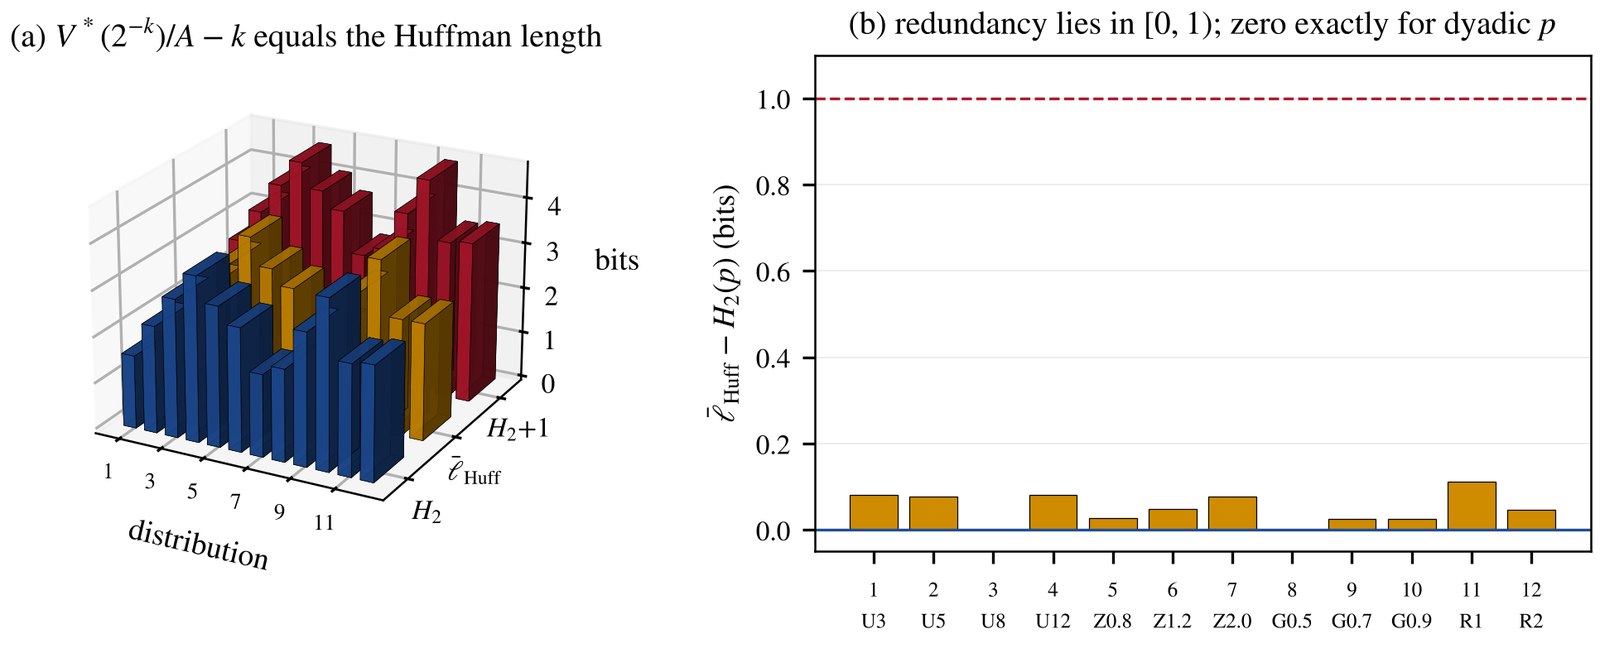
\includegraphics[width=0.98\textwidth]{figures/fig_huffman3d}
\caption{Theorem~\ref{thm:C} on twelve profiles: uniform on $3$, $5$, $8$ and $12$ candidates (U), Zipf with exponents $0.8$, $1.2$ and $2$ on ten (Z), geometric with ratios $0.5$, $0.7$ and $0.9$ on fourteen (G), and two random profiles on nine (R). (a) For each profile, the entropy $H_{2}(p)$, the optimal schedule cost $\Vs(2^{-k})/A-k$, which is the Huffman length, and $H_{2}(p)+1$. (b) The redundancy $\Vs/A-k-H_{2}(p)$, which lies in $[0,1)$; it vanishes on the dyadic profile, the uniform one on eight candidates (green), and is $2.7\times10^{-5}$ for the geometric profile of ratio one half, whose normalised weights differ from powers of two by the factor $2/(2-2^{-13})$. The largest redundancy, $0.112$, is that of the first random profile.}
\label{fig:huffman}
\end{figure*}

\begin{remark}[Larger alphabets]
For $D\ge3$ Huffman's algorithm merges the $D$ smallest weights at each step, after adding zero weights until $n\equiv1\pmod{D-1}$; the dummy candidates receive the longest codewords and cost nothing (Appendix~\ref{app:huffman}). A check of soundness $1/3$ run $r$ times is a ternary codeword of length $r$.
\end{remark}
